\chapter{Microservizio EventExport}
\label{cap:MicroservizioEventExport}

\section{Panoramica del microservizio}
\label{sec:ScopoDelMicroservizio}
Lo scopo del microservizio \textit{EventExport} è quello di elaborare dei \textbf{Business Event}, che arrivano dal microservizio \textit{EventEngine} 
(sezione \ref{subsubsec:event_engine}) e di comunicarli al cliente.\\\\
\textbf{EventExport} è configurabile in maniera differente per ogni cliente, di modo che ad un cliente vengano inviati solo alcuni tipi di eventi.
Ad esempio, un cliente potrebbe essere interessato solo agli eventi di creazione di un ordine, mentre un altro potrebbe voler ricevere tutti gli aggiornamenti
riguardo alla posizione dell'ordine da lui effettuato.
Questa configurazione è gestita tramite una tabella \textit{TradingPartnerEventLookup} che contiene le regole di filtro per ogni cliente.
\begin{figure}[htbp]
    \centering
    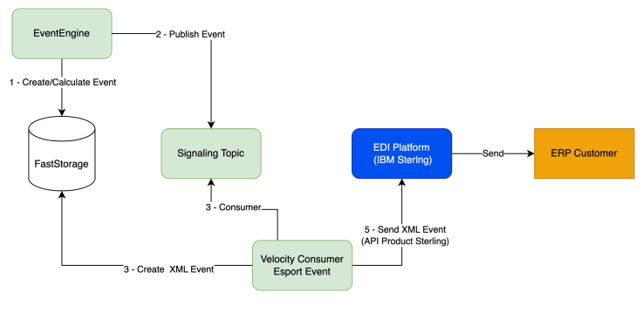
\includegraphics[width=\textwidth]{images/EventExport/EventExport_architecture.png}
    \caption{architettura con il microservizio \textit{EventExport}}
    \label{fig:EventExport_architecture}
\end{figure}\\
Il microservizio compie le seguenti operazioni:
\begin{enumerate}
    \item Consumare il \textit{Signaling Topic} (topic Kafka) applicando un filtro basato su una tabella di configurazione.
    \item Controllare se l'evento deve essere inviato. Non è necessario inviare eventi già inviati a meno di modifiche su campi significati 
    (anche questi definiti in base alla configurazione).
    \item Creare un file XML con i dati richiesti dal cliente. I dati sono definiti in base a dei template che vengono compilati in base alla configurazione.
    \item Inviare il file XML ad un altro servizio che si occuperà di inviare al cliente una mail.
    \item Loggare l'evento, compreso di XML, in una tabella (\textit{TransportOrdersExportEvents}) per tenere traccia degli eventi inviati.
\end{enumerate}


\section{Lettura del Signaling Topic}
\label{sec:LetturaDelSignalingTopic}
La lettura del \textit{Signaling Topic} avviene tramite un \textit{Consumer} Kafka.
Flink mette a disposizione un \textit{Kafka Consumer} 
che permette agevolmente di leggere i messaggi da un topic Kafka: \texttt{org.apache.flink.connector.kafka.source.KafkaSource}
Il \textit{Broker} Kafka su cui vive il \textit{Signaling Topic} è configurato per usare un sistema di autenticazione basato su \textit{SASL/SSL},
inoltre gli eventi sul topic sono serializzati tramite \textit{Apache Avro} (sezione \ref{subsec:avro_overview}) quindi è necessario configurare il \textit{Consumer Kafka} di conseguenza.
\begin{code}
    \inputminted[linenos]{java}{listings/EventsExport/KafkaSources.java}
    \caption{Configurazione del Kafka Consumer}
    \label{lst:KafkaSources}
\end{code}
Come mostrato nel codice \ref{lst:KafkaSources}, il \textit{Consumer Kafka} è configurato per leggere i messaggi dal topic \textit{Signaling Topic} 
ed il deserializzatore utilizzato è\\ \texttt{org.apache.flink.api.common.serialization.DeserializationSchema},
una classe messa a disposizione da Flink per deserializzare i messaggi \textit{Avro}.
Le righe 15,18,19 e 26 sono tipiche di un \textit{Consumer Kafka} scritto con \textit{Flink}, è presente infatti la creazione del \textit{builder} (riga 15),
la definizione del \textit{topic} da cui leggere (riga 18), l'offset da cui iniziare a leggere (riga 19) e  la creazione del \textit{Consumer} (riga 26).
Invece nelle righe 16 e 20-21 si possono leggere rispettivamente la configurazione del \textit{Kafka Consumer} e la configurazione del deserializzatore \textit{Avro}.\\\\
Nella chiamata alla funzione \texttt{forSpecific} a riga 21 i parametri sono la classe in cui verrà deserializzato il messaggio, l'url dello \textit{Schema Registry}
e le properties contenenti credenziali per accedere allo \textit{Schema Registry}. 
La configurazione del \textit{Kafka Consumer} e del deserializzatore \textit{Avro} è definita in un file \textit{.properties} e principalmente contiene
l'url dell'endpoint, le credenziali e diversi parametri per la connessione.
In un caso (\textit{Kafka}) è riferita al \textit{Broker Kafka} e nell'altro allo \textit{Schema Registry} (\textit{Avro}).

\section{Lettura della tabella di configurazione}
\label{sec:LetturaDellaTabellaDiConfigurazione}
La tabella di configurazione è una tabella \textit{SQL} chiamata \textit{TradingPartnerEventLookup} e contiene le regole di filtro per ogni cliente.
La connessione al database è gestita tramite \textit{JPA} e la libreria \textit{Hibernate} (sezione \ref{subsec:hibernate_overview}) con un sistema di caching
per evitare richieste ripetute al database. La cache viene aggiornata ogni ora.
\begin{table}[!ht]
    \centering
    \resizebox{\columnwidth}{!}{%
    \begin{tabular}{|l|l|l|l|l|l|l|l|}
    \hline
        Id & TradingPartner & OT & ERP & ID & Depot & Active & QueryCondition \\ \hline
        1 & TEST\_1 & 5 & 08 & null & null & Y & null \\ \hline
        2 & TEST\_1 & 5 & 20 & null & null & Y & null \\ \hline
        3 & TEST\_1 & 5 & 21 & null & null & Y & null \\ \hline
        4 & TEST\_1 & 5 & GEO & null & null & Y & null \\ \hline
        5 & TEST\_2 & 1 & COR & null & null & Y & null \\ \hline
        6 & TEST\_2 & 1 & GEN & null & null & Y & null \\ \hline
        7 & TEST\_3 & 5 & 10 & null & null & Y & null \\ \hline
        8 & TEST\_4 & 1 & COR & null & null & Y & null \\ \hline
        9 & TEST\_4 & 1 & VIC & null & null & Y & null \\ \hline
        10 & TEST\_4 & 1 & VSC & null & null & Y & null \\ \hline
        11 & TEST\_5 & 1 & CMG & null & null & Y & null \\ \hline
        12 & TEST\_5 & 1 & CMO & null & null & Y & null \\ \hline
        13 & TEST\_5 & 1 & CMR & null & null & Y & null \\ \hline
        14 & TEST\_5 & 1 & COR & null & null & Y & null \\ \hline
        15 & TEST\_5 & 1 & ERR & null & null & Y & null \\ \hline
        16 & TEST\_5 & 1 & GIA & null & null & Y & null \\ \hline
        17 & TEST\_5 & 1 & OAC & null & null & Y & null \\ \hline
        18 & TEST\_5 & 1 & STC & null & null & Y & null \\ \hline
    \end{tabular}%
    }
    \caption{Tabella TradingPartnerEventLookup di esempio}
    \label{tab:TradingPartnerEventLookup}
\end{table}
La tabella \ref{tab:TradingPartnerEventLookup} è un esempio di come potrebbe essere configurato il microservizio per inviare eventi a diversi clienti, I campi più rilevanti sono:
\begin{itemize}
    \item \textbf{TradingPartner}: il nome del cliente, in questo caso sono tutti clienti fittizi di test.
    \item \textbf{OT}: \textit{BusinessObjectType} il tipo di evento (1 Spedizione – 2 Ritiro – 5 Ordini).
    \item \textbf{ERP}: Lo specifico evento, ad esempio \textit{08} è l'evento di creazione di un ordine, \textit{GEO} è l'evento di modifica della posizione di un ordine.
    \item \textbf{Active}: se il filtro è attivo.
\end{itemize}

\textit{Flink} è basato sulla computazione distribuita di stream di dati (vedasi sezione \ref{sec:flink_overview}),
ciò va tenuto durante la creazione della cache per la tabella di configurazione. 
Infatti implementando una semplice cache locale (attraverso una \texttt{HashMap} ad esempio), si potrebbero avere problemi di consistenza dei dati e di sincronizzazione tra i vari nodi.
Inoltre tale implementazione non sfrutta le potenzialità di \textit{Flink} e la sua gestione automatica della scalabilità.
Per mostrare le problematiche di una cache implementata in maniera non corretta, si consideri il seguente esempio:\\
All'interno di un \textit{job}  viene creato un metodo che legge la tabella di configurazione e la memorizza in una \texttt{HashMap}, ogni 10 minuti la cache viene aggiornata.
Automaticamente il \textit{job} viene scalato su più nodi da \textit{Flink}, ogni nodo avrà la sua copia della cache e tale cache verrà aggiornata in maniera indipendente.
Questo comporta prima di tutto un problema di consistenza dei dati, in quanto un nodo potrebbe avere una copia della cache diversa 
qualora fosse impegnato in una computazione al momento dell'aggiornamento.
Ma soprattutto ogni nodo effettua una query al database in fase di aggiornamento, causando una serie di richieste tutti identiche e quindi ridondanti.
Se ad esempio il \textit{job} viene scalato su 10 nodi, ci saranno 10 richieste al database ad ogni aggiornamento, quando invece ne basterebbe una sola.\\\\
Il modo corretto di gestire questa cache è di utilizzare un datastream che legga la tabella di configurazione e la mantenga aggiornata, in collaborazione con il pattern 
\textbf{Broadcast State Pattern} per la distribuzione della cache tra i vari nodi.

\subsection{Rules Based Stream Processing}
\label{subsec:RulesBasedStreamProcessing}
Il \textit{Broadcast State Pattern} è un pattern di \textit{Flink} che permette di distribuire uno stato tra tutti i nodi di un job.
Questo stato è distribuito in maniera efficiente e scalabile, inoltre è possibile aggiornarlo in maniera asincrona.
Il \textit{Broadcast State Pattern} è fondamentale per la creazione di un sistema di \textit{Rules Based Stream Processing}, 
cioè un sistema che applica delle regole ad un flusso di dati.\\
Ci sono quindi due flussi di dati, uno contenente le regole e l'altro i dati a cui applicare le regole.
Ogni nodo mantiene un \textit{Broadcast State}, cioè una mappa che viene aggiornata all'arrivo di nuove regole.
Quando una nuova regola arriva dalla sorgente del flusso di regole, questa viene distribuita a tutti i nodi che andranno ad aggiornare il loro \textit{Broadcast State}
con la nuova regola, secondo quanto definito nel codice. In questo modo ogni nodo ha sempre una copia aggiornata delle regole da poter confrontare con i dati in arrivo sul flusso principale.
Quando invece un dato arriva sul flusso principale questi viene direttamente analizzato dal nodo che, eventualmente avvalendosi del \textit{Broadcast State}, lo elabora 
secondo quanto definito dalla logica implementativa.\\\\
Ad esempio (\todo{esempio preso dala documentazione di FLink, citarlo}), se una compagnia volesse analizzare le abitudini di acquisto su un e-commerce dei loro clienti 
potrebbe avvalersi di un \textit{Rules Based Stream Processing}. Quindi si avrebbero due stream, uno contenente tutte le operazioni svolte da un utente,
l'altro contenente il pattern che vogliamo analizzare, come mostrato in figura \ref{fig:broadcastState1}.
\begin{figure}[H]
    \centering
    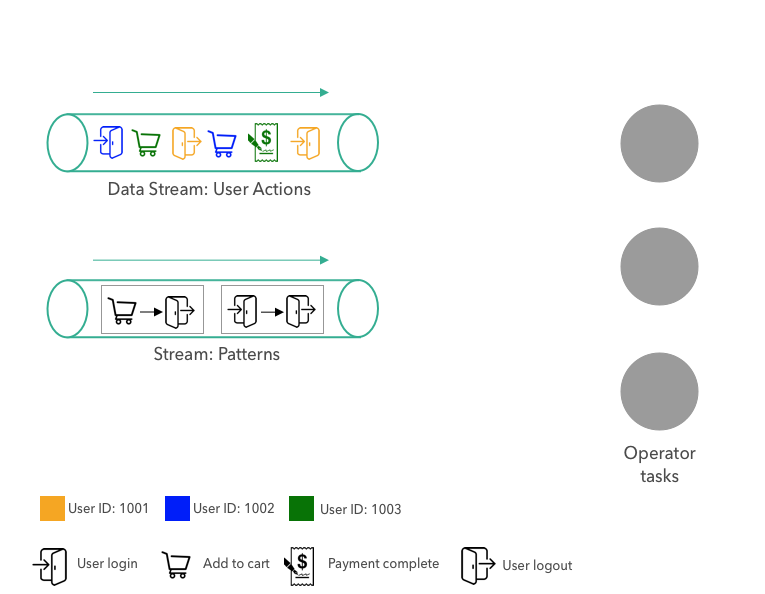
\includegraphics[width=0.7\textwidth]{images/EventExport/broadcastState1.png}
    \caption{Stream di dati e stream di regole}
    \label{fig:broadcastState1}
\end{figure}
Appena arriva una nuova regola, questa viene distribuita a tutti i nodi, che aggiorneranno i loro \textit{Broadcast State}.
Nel caso in figura \ref{fig:broadcastState2} ad esempio, il pattern appena giunto è l'operazione di ingresso al sito seguita da un'uscita, senza acquisti.
\begin{figure}[H]
    \centering
    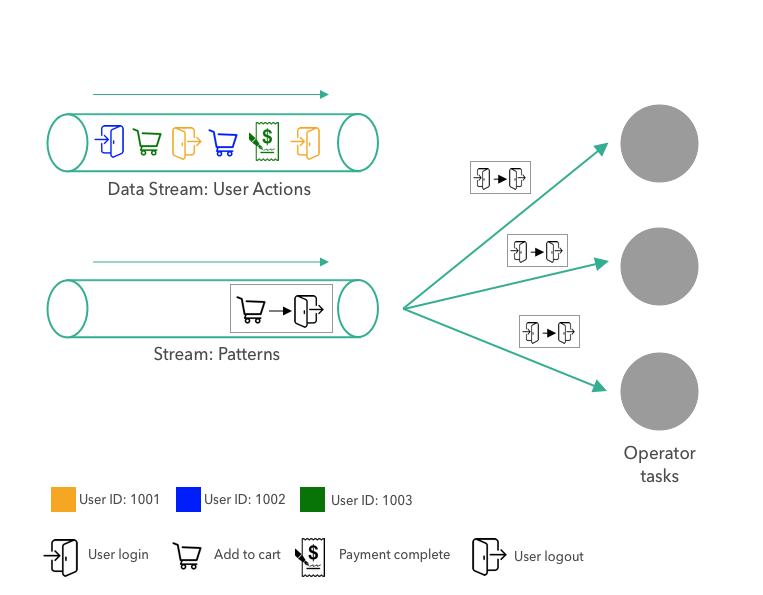
\includegraphics[width=0.7\textwidth]{images/EventExport/broadcastState2.png}
    \caption{Aggiornamento del \textit{Broadcast State}}
    \label{fig:broadcastState2}
\end{figure}
Successivamente, quando arriva un nuovo dato, questo viene analizzato dal nodo che, avvalendosi del \textit{Broadcast State}, lo elabora secondo quanto definito dalla regola.
Ad esempio nella sezione sinistra della figura \ref{fig:broadcastState3/4}, si può notare che viene ricevuto il seguente dato \textit{il cliente 1001 entra nel sito}.
Nel frattempo gli altri due clienti effettuano altre operazioni che vengono inviate ai relaviti nodi.
Successivamente arriva un altro dato \textit{il cliente 1001 esce dal sito} (parte destra della figura), che viene inviato al primo nodo.
Questo nodo, avendo memoria della regola impostata nel \textit{Broadcast State}, riconosce il pattern e lo invia al sistema di analisi.
\begin{figure}[H]
    \centering
    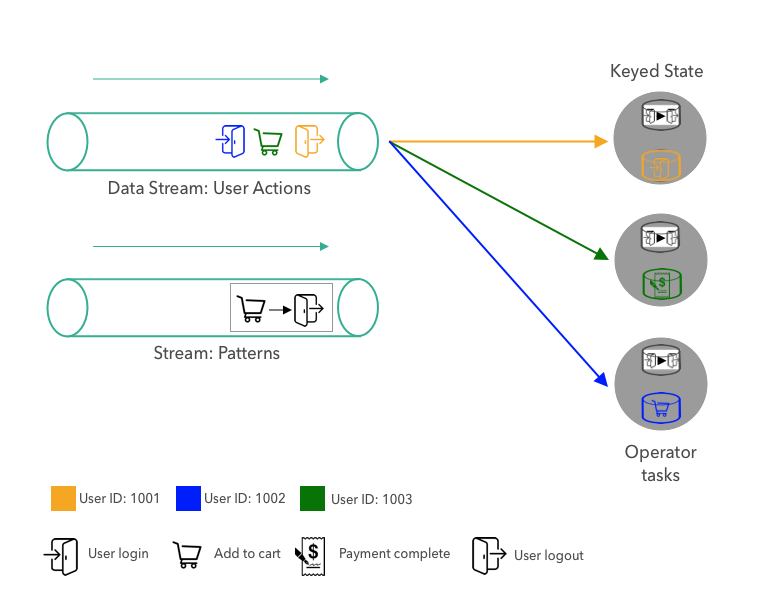
\includegraphics[width=0.49\textwidth]{images/EventExport/broadcastState3.png}
    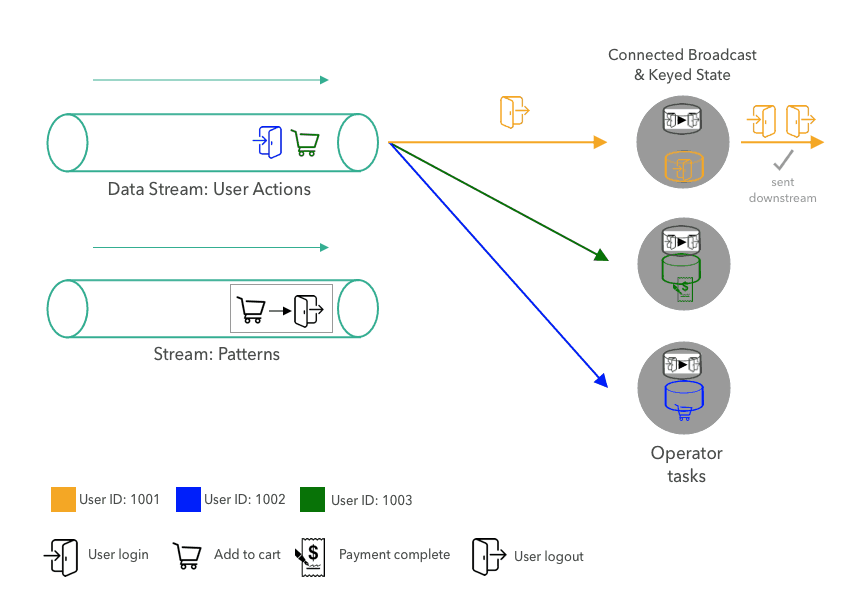
\includegraphics[width=0.49\textwidth]{images/EventExport/broadcastState4.png}
    \caption{Esempio di pattern riconosciuto}
    \label{fig:broadcastState3/4}
\end{figure}



\subsection{Implementazione del Rules Based Stream Processing}
\label{subsec:ImplementazioneDelRulesBasedStreamProcessing}
Come descritto in precedenza (sezione \ref{subsec:RulesBasedStreamProcessing}), il Rules Based Stream Processing è un sistema che applica delle regole ad un flusso di dati.
In questo caso le regole sono quelle contenute nella tabella \textit{TradingPartnerEventLookup} e il flusso di dati è quello dei \textit{Business Event} provenienti dal \textit{Signaling Topic}.
